%\documentclass{article}
\documentclass[preview]{standalone}
%\usepackage{tikz}
\usepackage{pgfplots}
%\usepackage{subfigure}

\begin{document}

\newcommand\gauss[2]{1/(#2*sqrt(2*pi))*exp(-((x-#1)^2)/(2*#2^2))} 
\tikzstyle{place}=[circle,draw=blue!50,fill=blue!20,thick]


\begin{tikzpicture}[scale=0.5,cube/.style={very thin,black}]
    %\draw[step=1cm,gray,very thin] (-2,-2) grid (24,24);

    \node[inner sep=0cm] (gaussian) at (2.75,7.5)
        {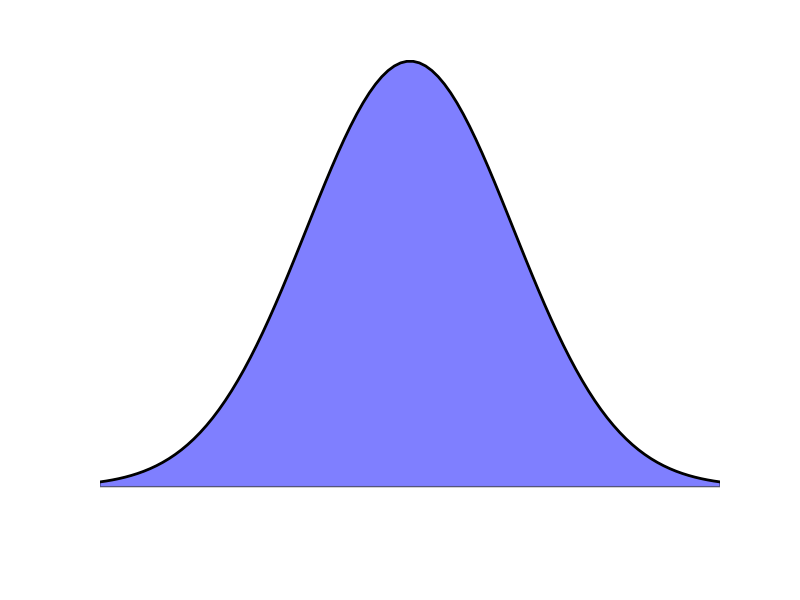
\includegraphics[width=.14\textwidth]{gaussian.png}};
    \node[inner sep=0cm] (gaussian) at (6.75,7.5)
        {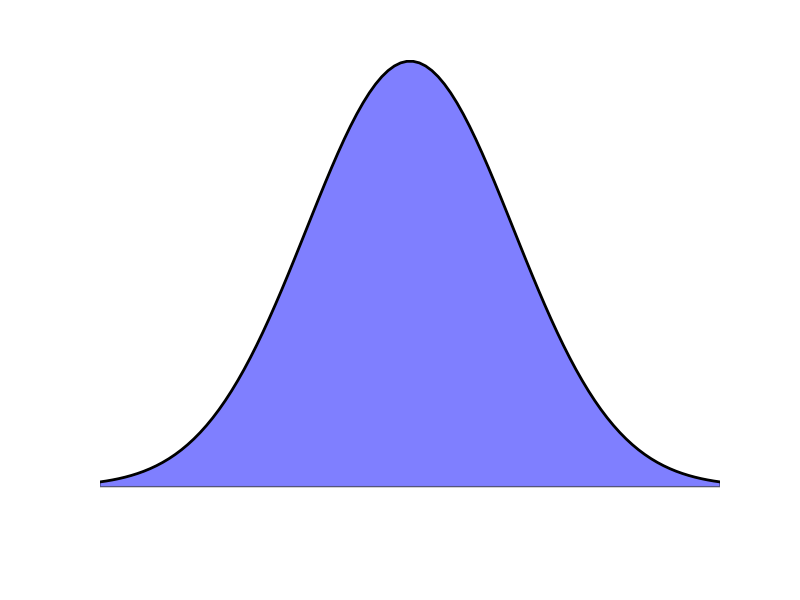
\includegraphics[width=.14\textwidth]{gaussian.png}};
    \node[inner sep=0cm] (gaussian) at (10.75,7.5)
        {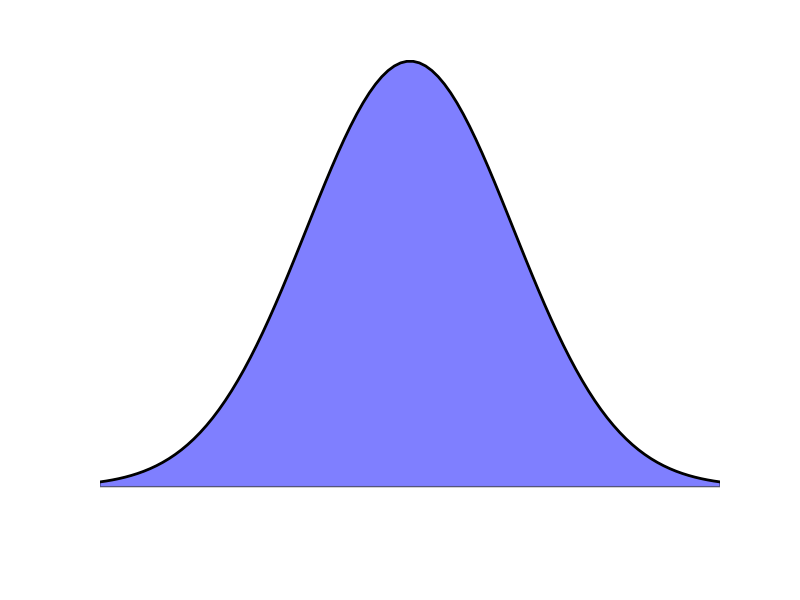
\includegraphics[width=.14\textwidth]{gaussian.png}};

    \node[inner sep=0cm] (gaussian) at (1.5,17.5)
        {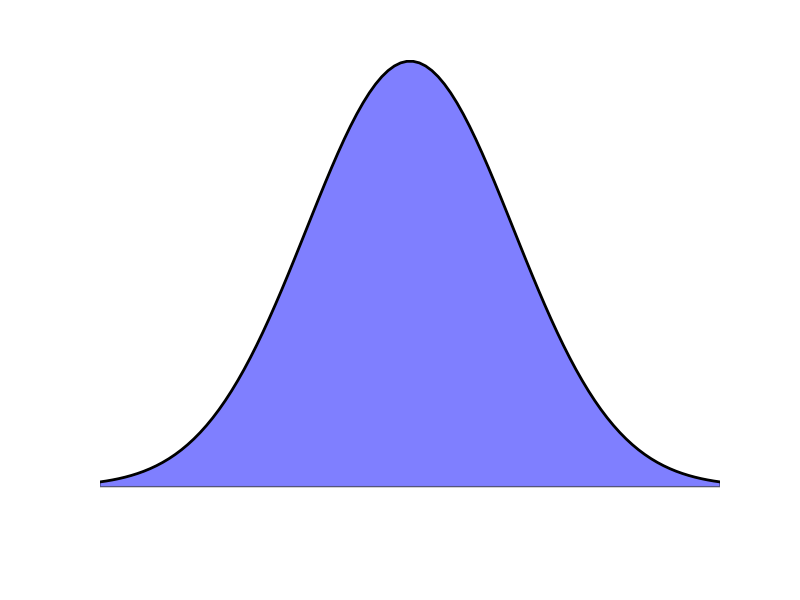
\includegraphics[width=.05\textwidth]{gaussian.png}};
    \node[inner sep=0cm] (gaussian) at (2.5,17.5)
        {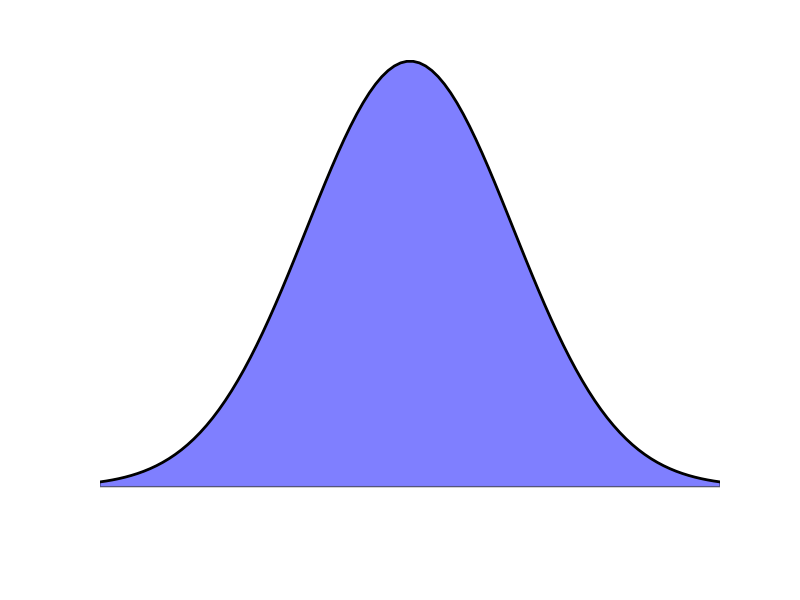
\includegraphics[width=.05\textwidth]{gaussian.png}};
    \node[inner sep=0cm] (gaussian) at (3.5,17.5)
        {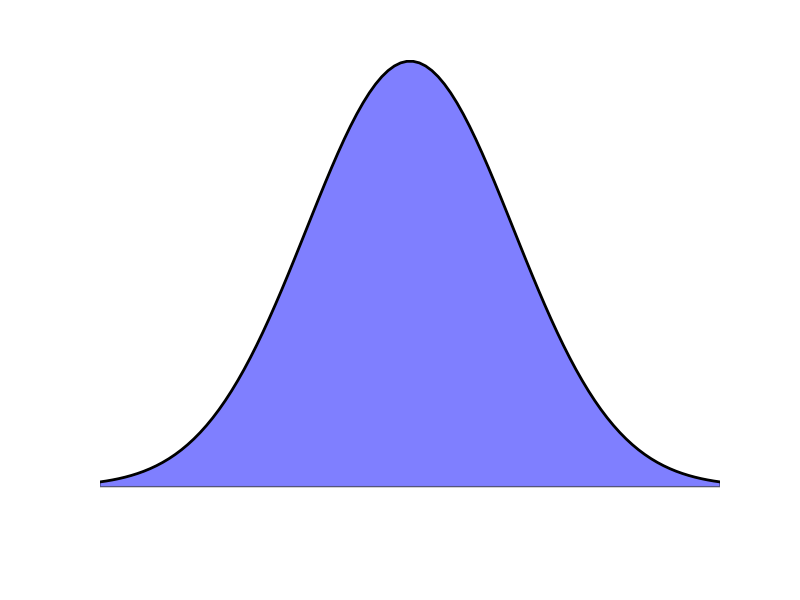
\includegraphics[width=.05\textwidth]{gaussian.png}};

    \node[inner sep=0cm] (gaussian) at (5.5,17.5)
        {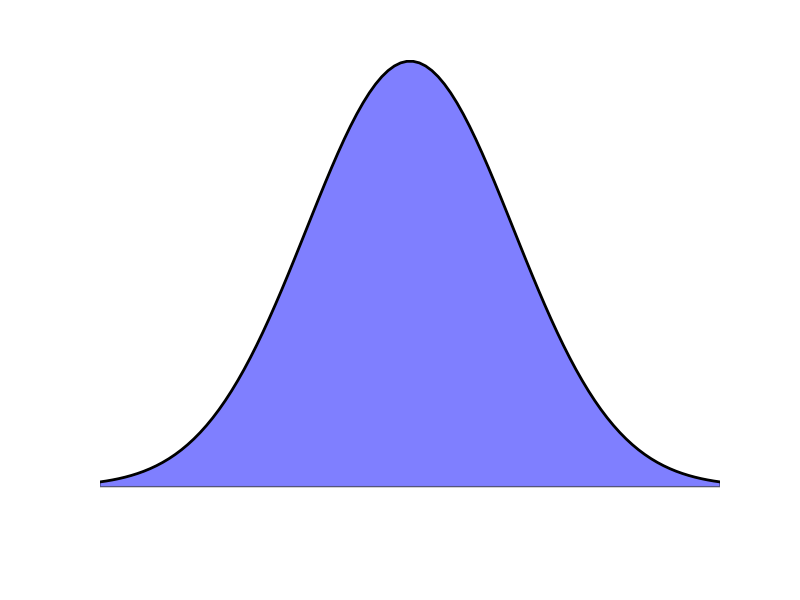
\includegraphics[width=.05\textwidth]{gaussian.png}};
    \node[inner sep=0cm] (gaussian) at (6.5,17.5)
        {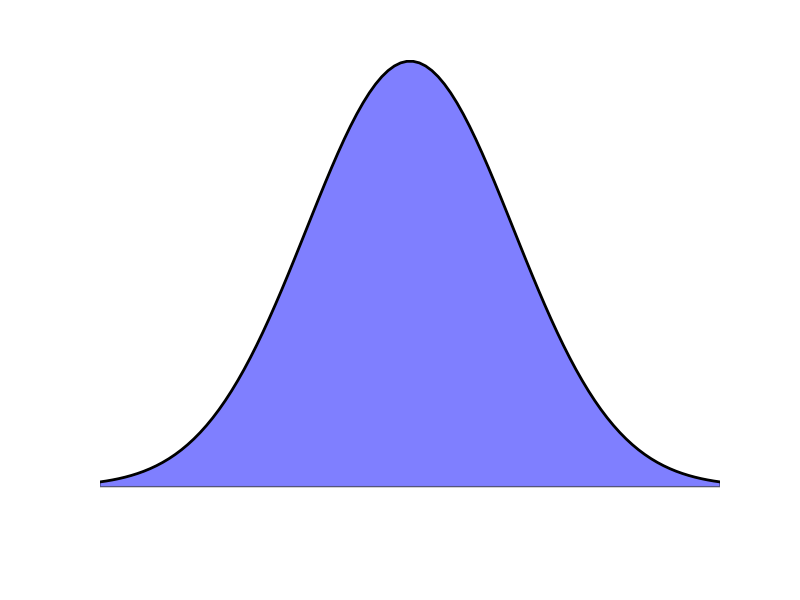
\includegraphics[width=.05\textwidth]{gaussian.png}};
    \node[inner sep=0cm] (gaussian) at (7.5,17.5)
        {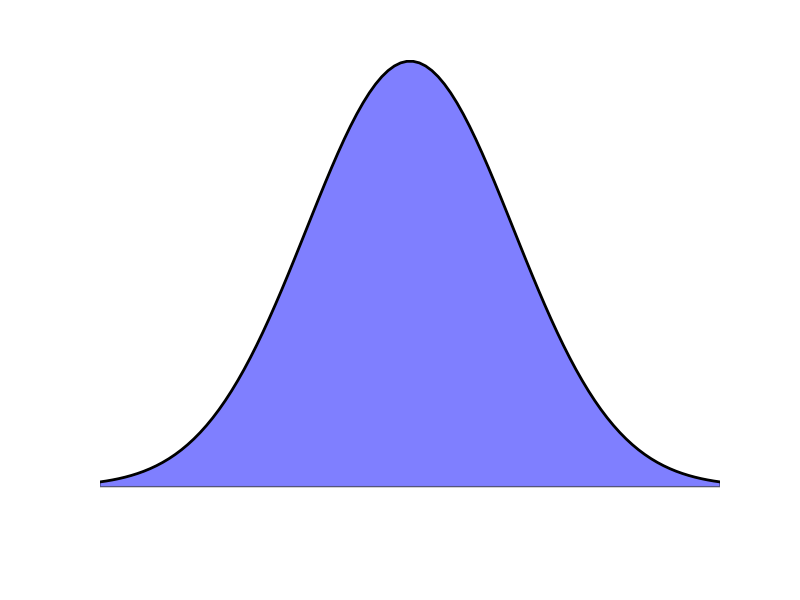
\includegraphics[width=.05\textwidth]{gaussian.png}};

    \node[inner sep=0cm] (gaussian) at (9.5,17.5)
        {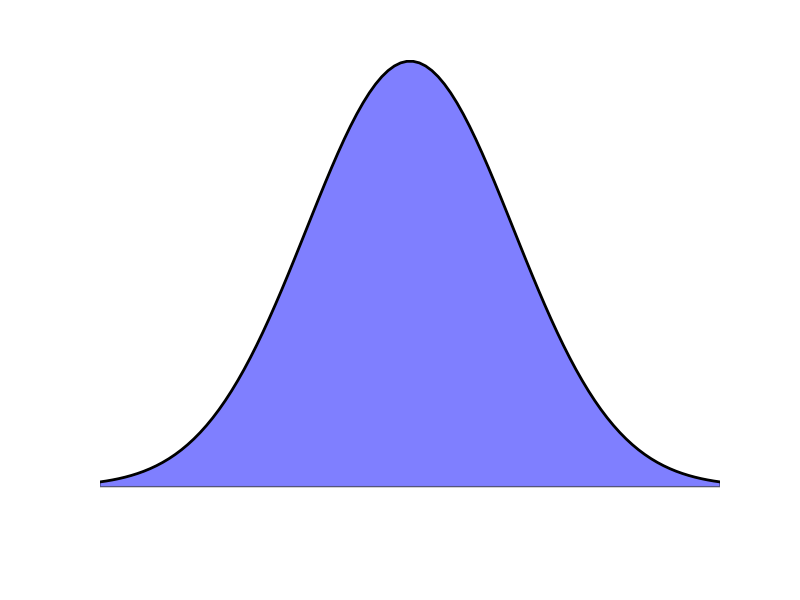
\includegraphics[width=.05\textwidth]{gaussian.png}};
    \node[inner sep=0cm] (gaussian) at (10.5,17.5)
        {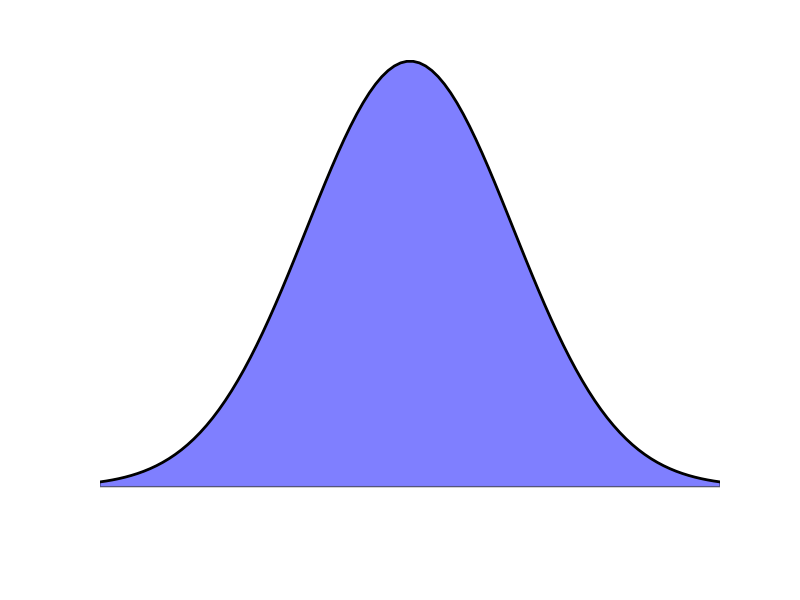
\includegraphics[width=.05\textwidth]{gaussian.png}};
    \node[inner sep=0cm] (gaussian) at (11.5,17.5)
        {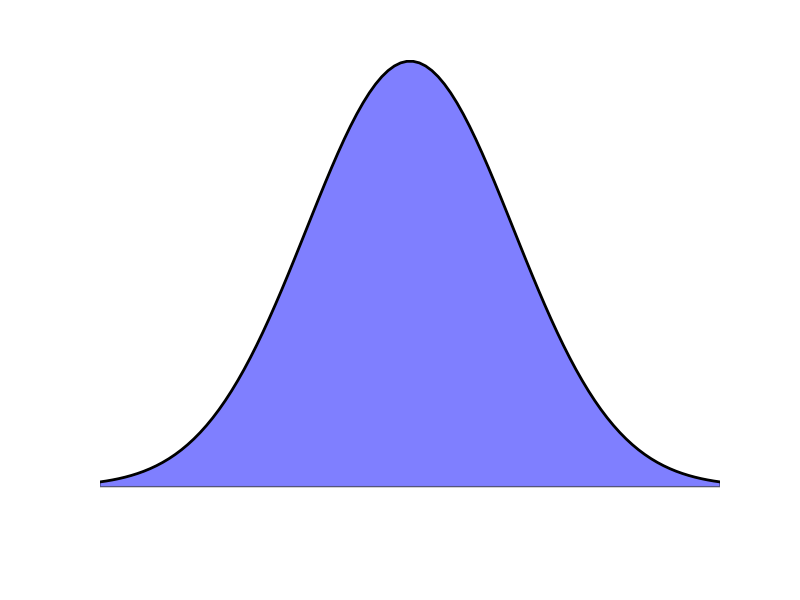
\includegraphics[width=.05\textwidth]{gaussian.png}};

    % First rectangle
    \draw (5,0) rectangle (8.5,3);
    \draw [fill=blue]   (5.5,1) rectangle (6,2);
    \draw [fill=green] (6.5,1) rectangle (7,2);
    \draw [fill=red]     (7.5,1) rectangle (8,2);

    % First gaussian filter
    \draw (1,6) rectangle (4.5,9);
    \draw (5,6) rectangle (8.5,9);
    \draw (9,6) rectangle (12.5,9);

    \draw [->,blue] (1.75,6) -- (2,5);
    \draw [->,blue] (2.75,6) -- (2.75,5.35);
    \draw [->,blue] (3.75,6) -- (3.5,5);
    \draw [->,blue] (2.75,4.5) -- (5,3);

    \draw [->,red] (9.75,6) -- (10,5);
    \draw [->,red] (10.75,6) -- (10.75,5.35);
    \draw [->,red] (11.75,6) -- (11.5,5);
    \draw [->,red] (10.75,4.5) -- (8.5,3);

    \draw [->,green] (5.75,6) -- (6,5);
    \draw [->,green] (6.75,6) -- (6.75,5.35);
    \draw [->,green] (7.75,6) -- (7.5,5);
    \draw [->,green] (6.75,4.5) -- (6.75,3);


    % middle rectangles 
    \draw (1,12) rectangle (4.5,15);
    \draw (5,12) rectangle (8.5,15);
    \draw (9,12) rectangle (12.5,15);

    \draw [fill=blue]   (1.5,13) rectangle (2,14);
    \draw [fill=blue]   (2.5,13) rectangle (3,14);
    \draw [fill=blue]   (3.5,13) rectangle (4,14);

    \draw [fill=green]   (5.5,13) rectangle (6,14);
    \draw [fill=green]   (6.5,13) rectangle (7,14);
    \draw [fill=green]   (7.5,13) rectangle (8,14);

    \draw [fill=red]   (9.5,13) rectangle (10,14);
    \draw [fill=red]   (10.5,13) rectangle (11,14);
    \draw [fill=red]   (11.5,13) rectangle (12,14);

    % small filter rectangles
    \draw (1,17) rectangle (2,18);
    \draw (2,17) rectangle (3,18);
    \draw (3,17) rectangle (4,18);

    \draw (5,17) rectangle (6,18);
    \draw (6,17) rectangle (7,18);
    \draw (7,17) rectangle (8,18);

    \draw (9,17) rectangle (10,18);
    \draw (10,17) rectangle (11,18);
    \draw (11,17) rectangle (12,18);

    % mult. rectangles and nodes
    \node at ( 2.75,10.5) [place] {$(*)$};
    \node at ( 6.75,10.5) [place] {$(*)$};
    \node at ( 10.75,10.5) [place] {$(*)$};

    \node at ( 2.75,19.5) [place] {$(*)$};
    \node at ( 6.75,19.5) [place] {$(*)$};
    \node at ( 10.75,19.5) [place] {$(*)$};

    % arrows of multiple rectangle nodes
    \draw [->,blue] (1.5,17) -- (1.5,15);
    \draw [->,blue] (5.5,17) -- (2.75,15);
    \draw [->,blue] (9.5,17) -- (3.75,15);

    \draw [->,green] (2.5,17) -- (5.5,15);
    \draw [->,green] (6.5,17) -- (6.75,15);
    \draw [->,green] (10.5,17) -- (7.75,15);

    \draw [->,red] (3.5,17) -- (9.5,15);
    \draw [->,red] (7.5,17) -- (10.75,15);
    \draw [->,red] (11.5,17) -- (11.75,15);

    % rectangles
    \draw (1,21) rectangle (4.5,24);
    \draw (5,21) rectangle (8.5,24);
    \draw (9,21) rectangle (12.5,24);

    \draw [fill=blue]   (1.5,22) rectangle (2,23);
    \draw [fill=green]   (2.5,22) rectangle (3,23);
    \draw [fill=red]   (3.5,22) rectangle (4,23);

    \draw [fill=blue]   (5.5,22) rectangle (6,23);
    \draw [fill=green]   (6.5,22) rectangle (7,23);
    \draw [fill=red]   (7.5,22) rectangle (8,23);

    \draw [fill=blue]   (9.5,22) rectangle (10,23);
    \draw [fill=green]   (10.5,22) rectangle (11,23);
    \draw [fill=red]   (11.5,22) rectangle (12,23);


    % sum nodes
    \node at ( 2.75,4.5) [place] {$\sum$};
    \node at ( 6.75,4.5) [place] {$\sum$};
    \node at ( 10.75,4.5) [place] {$\sum$};


\end{tikzpicture}
\end{document}
